% Augmented Reality

\chapter{Augmented Reality} % Main chapter title

\label{AugmentedReality}

%----------------------------------------------------------------------------------------

This chapter covers the AR portion of the project. The AR subsystem takes the positions from the position calculation subsystem and renders them on the screen of a cellphone using OpenGL. If they cannot be directly rendered, an arrow is drawn on the edge of the screen to show which way the object is from the user. An example of this can be found in Figure~\ref{dfis} (DO THIS FIGURE).

The code for the AR subsystem can be found at (PROVIDE LINK HERE).

This chapter covers the following topics:
\begin{enumerate}
	\item A brief overview of the math used later in this section, including homogenous coordinates and translation/rotation matrices.
	\item A description of OpenGL and the basics of how it can be used. 
	\item How objects and text can accurately be drawn on the screen overlaid on a camera image.
	\item How the coordinate system of the position calculation system can be transformed into real world coordinates through the cell phone's sensors.
	\item Examples of the accuracy of the subsystem.
\end{enumerate}

\section{3D Math Overview}
This section covers the basics of using matrices to render 3D scenes. A full treatment of the subject is beyond the scope of this report, though other resources on the subject exist (PUT CITATION HERE).

\subsection{Transformation Matrices}

\subsection{Homogenous Coordinates}
For a given 3$\times$3 matrix $M$ and an arbitrary point in 3D space $p = (x, y, z)$, there is no $\mathbf{M}$ such that will multiplying it by any $p$ will cause $p$ to be translated by a specified number of units. There is, however, a way to do it with a homogenous point and a 4x4 matrix. This is one of the reasons homogenous coordinates are used in OpenGL.

Homogenous coordinates are coordinates in space which contain an extra element $w$ which acts as a scaling factor on the three elements. For example, a 3D homogenous coordinate $p_h$ could be written as:

\[ p_h = (x_h, y_h, z_h, w) \]

This relates to a regular point in 3D space:

\[ (x, y, z) = (x_h / w, y_h / w, z_h / w) \] 

For example, the homogenous point $(1, 1, 1, 1)$ maps to the regular 3D point $(1, 1, 1)$. The homogenous point $(2, 2, 2, 2)$ does as well.

A translation matrix $T$ that moves a point $p$  by $(T_x, T_y, T_z)$ units, is:

\[
\mathbf{T} = \begin{bmatrix}
1 & 0 & 0 & T_x \\
0 & 1 & 0 & T_y \\
0 & 0 & 1 & T_z \\
0 & 0 & 0 & 1
\end{bmatrix}
\]

To prove this, we'll multiply out a homogenous point $p_h = (x_h, y_h, z_h, w)$ by $\mathbf{T}$ and show that, when converted to a regular 3D point, it equals $(x/w + T_x, y/w + T_y, z/w + T_z)$.

\[ p_{h}\prime = \mathbf{T} p_h \]

\[
  p_{h}\prime = \begin{bmatrix}
1 & 0 & 0 & T_x \\
0 & 1 & 0 & T_y \\
0 & 0 & 1 & T_z \\
0 & 0 & 0 & 1
\end{bmatrix} 
\begin{bmatrix}
x_h \\ y_h \\ z_h \\ w 
\end{bmatrix}
\]

\[
 p_{h}\prime = \begin{bmatrix}
 x_h + w T_x \\
 y_h + w T_y \\
 z_h + w T_z \\
 w
 \end{bmatrix}
 \]
 
 Now, if we convert $p_{h}\prime$ to a regular 3D point $p$, we get:
 
 \[ p = (\frac{x_h}{w} + \frac{w T_x}{w},  \frac{y_h}{w} + \frac{w T_y}{w}, \frac{z_h}{w} + \frac{w T_z}{w}) \]
 \[ p = (x/w + T_x, y/w + T_y, z/w + T_z) \]
 
 which is the translation of $p$ by $(T_x, T_y, T_z)$ units.
 
 \section{OpenGL}
OpenGL is an API used to render 2D and 3D graphics. For the project, OpenGL was used to render position markers in 3D space overtop what the cell phone's camera sees.

OpenGL works by taking in collections of points making up a 3D model of an object and then applying various matrix transforms to the points, translating and rotating them. Afterwards, it projects them onto a 2D plane and renders them. A full treatment of how OpenGL works is beyond the scope of this report, but (INSERT CITATION HERE FOR OPENGL BOOK).

The three main matrices that OpenGL uses to render a 3D scene are called the \textbf{projection matrix}, \textbf{view matrix}, and \textbf{model matrix}. This project uses several novel techniques which use and manipulate the matrices that OpenGL uses to render a 3D scene. This report will only cover them briefly, though other resources explore them more fully \cite{CodingLabs}.

\section{The Model Matrix}
\begin{figure}
	\centering
	\tikzstyle{vertex}=[circle, draw]
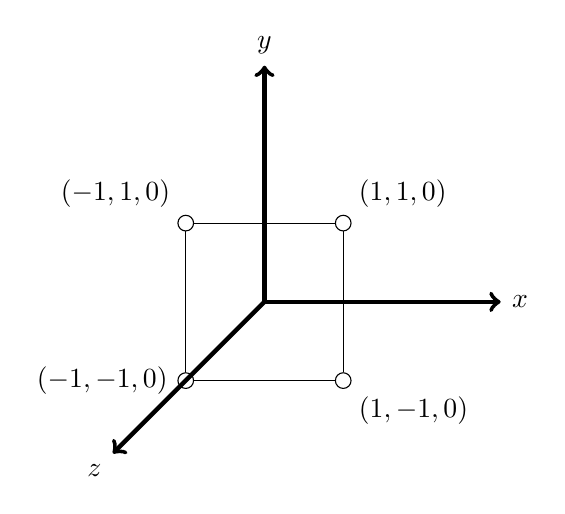
\begin{tikzpicture}[transform shape]
\draw[->,ultra thick] (0,0, 0)--(3,0, 0) node[right]{$x$};
\draw[->,ultra thick] (0,0, 0)--(0,3, 0) node[above]{$y$};
\draw[->,ultra thick] (0,0, 0)--(0,0, 5) node[below left]{$z$};

\node[vertex,inner sep=2pt,minimum size=1pt,label=left:{$(-1, -1, 0)$}](v1) at (-1, -1, 0) {};
\node[vertex,inner sep=2pt,minimum size=1pt,label=below right:{$(1, -1, 0)$}](v2) at (1, -1, 0) {};
\node[vertex,inner sep=2pt,minimum size=1pt,label=above right:{$(1, 1, 0)$}](v3) at (1, 1, 0) {};
\node[vertex,inner sep=2pt,minimum size=1pt,label=above left:{$(-1, 1, 0)$}](v4) at (-1,1, 0) {};

\begin{scope}[every path/.style={-}, every node/.style={inner sep=0pt}]
       \draw (v1) -- node [anchor=south east] {} (v2);
       \draw (v2) -- node [anchor=south west] {} (v3);
       \draw (v3) -- node [anchor=north] {} (v4);
       \draw (v4) -- node [anchor=north] {} (v1);
\end{scope} 
\end{tikzpicture}
	\decoRule
	\caption{An example 3D model of a square in model coordinates.}
	\label{fig:ModelExample}
\end{figure}
\begin{figure}
	\centering
	\tikzstyle{vertex}=[circle, draw]
\begin{tikzpicture}[transform shape={scale=0.4}]
\draw[->,ultra thick] (0,0, 0)--(5,0, 0) node[right]{$x$};
\draw[->,ultra thick] (0,0, 0)--(0,5, 0) node[above]{$y$};
\draw[->,ultra thick] (0,0, 0)--(0,0, 5) node[below left]{$z$};

\node[vertex,inner sep=2pt,minimum size=1pt,label=below:{$(-6, -1, 0)$}](v1) at (-6, -1, 0) {};
\node[vertex,inner sep=2pt,minimum size=1pt,label=below right:{$(-4, -1, 0)$}](v2) at (-4, -1, 0) {};
\node[vertex,inner sep=2pt,minimum size=1pt,label=above right:{$(-4, 1, 0)$}](v3) at (-4, 1, 0) {};
\node[vertex,inner sep=2pt,minimum size=1pt,label=above:{$(-6, 1, 0)$}](v4) at (-6,1, 0) {};

\node[vertex,inner sep=2pt,minimum size=1pt,label=left:{$(4, -1, 0)$}](v5) at (4, -1, 0) {};
\node[vertex,inner sep=2pt,minimum size=1pt,label=below right:{$(6, -1, 0)$}](v6) at (6, -1, 0) {};
\node[vertex,inner sep=2pt,minimum size=1pt,label=above right:{$(6, 1, 0)$}](v7) at (6, 1, 0) {};
\node[vertex,inner sep=2pt,minimum size=1pt,label=above left:{$(4, 1, 0)$}](v8) at (4,1, 0) {};

\begin{scope}[every path/.style={-}, every node/.style={inner sep=0pt}]
       \draw (v1) -- node [anchor=south east] {} (v2);
       \draw (v2) -- node [anchor=south west] {} (v3);
       \draw (v3) -- node [anchor=north] {} (v4);
       \draw (v4) -- node [anchor=north] {} (v1);
       
       \draw (v5) -- node [anchor=south east] {} (v6);
       \draw (v6) -- node [anchor=south west] {} (v7);
       \draw (v7) -- node [anchor=north] {} (v8);
       \draw (v8) -- node [anchor=north] {} (v5);
\end{scope} 
\end{tikzpicture}
	\decoRule
	\caption{A 3D scene with two squares, the centers of which are placed at $(5, 0, 0)$ and $(-5, 0, 0)$ in world coordinates by transforming the vertices of Figure~\ref{fig:ModelExample} with two model matrices.}
	\label{fig:ModelMatrixExample}
\end{figure}

The model matrix exists to take \textbf{model space}, in which the coordinates of a 3D model are relative to the center of the model, and transform it into \textbf{world space}, in which coordinates are relative to the center of the ``world''. Most of the code in this project considers the locations of objects in world space. For example, the position subsystem might say that a tag is at $(5, 5, 1)$. This coordinate is considered to be in world space, though it should be noted that this is not the same as \emph{real} world coordinates - a further transform is required to match up the positions given by the position calculation subsystem with the real world as shown by a camera.

Figure~\ref{fig:ModelExample} shows an example of a square in model space. The square's 3D model has its vertices placed at $(-1, -1, 0)$, $(1, -1, 0)$, $(1, 1, 0)$, and $(-1, 1, 0)$. An example of creating a 3D scene with two squares at $(5, 0, 0)$ and $(-5, 0, 0)$ in world coordinates can be seen in Figure~\ref{fig:ModelMatrixExample}. A model matrix is created for each of the squares. The first model matrix encodes a translation $(-5, 0, 0)$ units and the second model matrix encodes a translation of $(5, 0, 0)$ units. To get the vertices of the first square in world coordinates, the first model matrix is applied to the square's vertices. The same is done for the second square and model matrix. 

That is, for the model matrix $\mathbf{M}$ and each vertex $v$ of the square, the vertex $v$ is transformed into world coordinates vertex $v'$ by the formula:

\[v' = \mathbf{M}v \]

\section{The View Matrix}
\begin{figure}
	\centering
	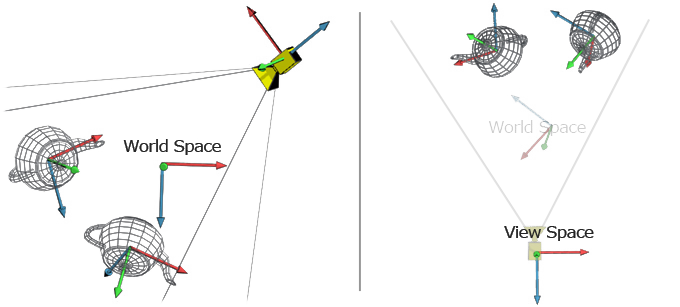
\includegraphics[width=\linewidth]{Figures/WorldToView.png}
	\decoRule
	\caption{A figure showing an object in world coordinates and an object in camera coordinates \cite{CodingLabs}.}
	\label{fig:WorldToView}
\end{figure}

In a 3D scene, a position is declared from which the scene is viewed. The view matrix exists to transform world coordinates to \textbf{view space}, in which coordinates are relative to the position from which the scene is viewed. It as if an imaginary camera has been placed in the scene. Figure~\ref{fig:WorldToView} shows an example of this.

The view matrix is typically just a simple translation of all the vertices (if a camera is placed at $(5, 5, 5)$, then all the vertices will be translated by $(-5, -5, -5)$), and then a rotation based in which direction the camera is looking at. 

For the rest of this project, the imaginary camera is assumed to be located at (0, 0, 0), making the view matrix a simple rotation matrix. The positions of markers and objects are calculated relative to the position of the tag connected to the cellphone.

\section{The Projection Matrix}

\begin{figure}
	\centering
	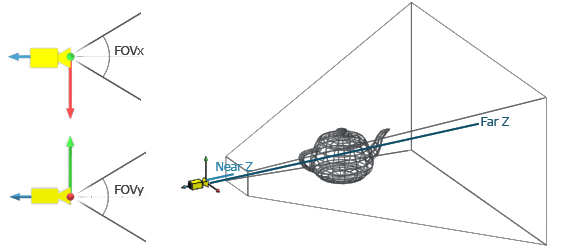
\includegraphics[width=\linewidth]{Figures/ProjectionMatrix.png}
	\decoRule
	\caption{The transformation from view space to projection space \cite{CodingLabs}.}
	\label{fig:ProjectionMatrix}
\end{figure}

\begin{figure}
	\centering
	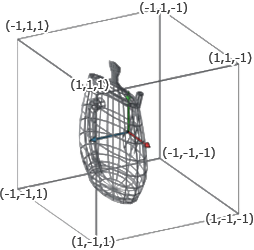
\includegraphics{Figures/ProjectionMatrix2.png}
	\decoRule
	\caption{A teapot in projection space \cite{CodingLabs}.}
	\label{fig:ProjectionMatrix2}
\end{figure}

In one of the last steps in rendering a 3D scene in OpenGL, the scene must be projected onto a plane so it can be displayed on a monitor. The projection matrix is involved in this process. View space is transformed into \textbf{projection space}, in which coordinates are transformed into \textbf{normalized device coordinates} (NDCs). Vertices which fall within the field of view will be contained within a cube with corners $(-1, -1, -1)$ and $(1, 1, 1)$ and are drawn. Vertices outside this box are culled. 

There are different types of projection matrices. For the purposes of this projection, only the \textbf{perspective projection matrix} is considered. This projection takes into account that objects which are further away from the camera should appear smaller. Figure~\ref{fig:ProjectionMatrix} and Figure~\ref{fig:ProjectionMatrix2} show the transform from view space to projection space via a perspective projection matrix.

To actually render the image in 2D, the NDCs are converted to the coordinates of pixels as determined by the size of the surface being rendered to. The $z$ coordinates handle depth, which allows OpenGL to determine whether a shape is on top of another during the rendering process.

\section{Camera Perspective and OpenGL Perspective}
\begin{figure}
	\centering
	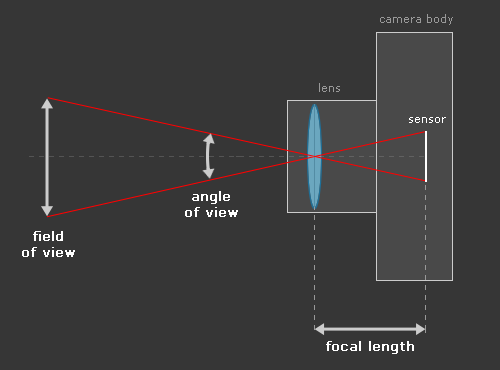
\includegraphics[width=\linewidth]{Figures/CameraLens.png}
	\decoRule
	\caption{A diagram depicting the field of view of a camera \cite{MartyBugs}.}
	\label{fig:CameraLens}
\end{figure}
In order to accurately display the locations of the devices, it is important that the 3D scene rendered by OpenGL match up with the real world as shown by the cellphone's camera. Figure~\ref{fig:CameraLens} shows how a camera can only see see a limited part of the world, as dictated by its field of view.

As previously shown in Figure~\ref{ProjectionMatrix}, the projection matrix has a field of view which can be changed. The field of view for the OpenGL perspective matrix needs to be set on a per-cellphone basis to match that of the cellphone's camera for the project to display locations accurately.

\section{Cellphone Rotation}
Discuss in detail more about how Android implements getting the rotation, the limits of it when moving + in strong magnetic fields.

\section{Billboard Effect}
Talk about how doing the inverted view matrix multiplication causes things to always face the screen. Give pictures! Motivation here is to make 2D images that we can place in 3D space and have them face the screen.

\section{HUD}
Go over how the HUD is made. (Still need to finish that too so we can get pictures.)

\section{Calibration}
Talk about how we can take the cellphone's rotation matrix and calibrate the positions we calculate from anchors/tags.

\section{Results}
Show off how accurate we are. Have Youtube videos displaying such.

\section{Conclusion}
Conclusion of this section: we can render positions on the screen and have 3D math to do so etc.
